\documentclass[a4paper,10pt]{article}
\usepackage[utf8]{inputenc}

% ----  Useful packages % ---- 
\usepackage{amsmath}
\usepackage{graphicx}
\graphicspath{{./images/}}
\usepackage{amsfonts}
\usepackage{amsthm}
\usepackage{amssymb}
\usepackage{makecell}
% ----  Useful packages % ---- 

\usepackage{wrapfig}
\usepackage{caption}
\usepackage{subcaption}
\usepackage{hyperref}
\hypersetup{
	colorlinks,
	citecolor=black,
	filecolor=black,
	linkcolor=black,
	urlcolor=black
}

% ---- Set page size and margins replace ------
\usepackage[letterpaper,top=2cm,bottom=2cm,left=3cm,right=3cm,marginparwidth=1.75cm]{geometry}
% ---- Set page size and margins replace ------

% ------- NOTA ------
\theoremstyle{remark}
\newtheorem{note}{Note}[subsection]
% ------- NOTA ------

% ------- OSSERVAZIONE ------
\theoremstyle{definition}
\newtheorem{observation}{Osservazione}[subsection]
% ------- OSSERVAZIONE ------

% ------- DEFINIZIONE ------
\theoremstyle{plain}
\newtheorem{definition}{Definizione}[subsection]
% ------- DEFINIZIONE ------

% ------- ESEMPIO ------
\theoremstyle{definition}
\newtheorem{example}{Esempio}[subsection]
% ------- ESEMPIO ------

% ------- DIMOSTRAZIONE ------
\theoremstyle{definition}
\newtheorem{demostration}{Dimotrazione}[subsection]
% ------- DIMOSTRAZIONE ------

% ------- TEOREMA ------
\theoremstyle{definition}
\newtheorem{theorem}{Teorema}[subsection]
% ------- TEOREMA ------

% ------- COROLLARIO ------
\theoremstyle{plain}
\newtheorem{corollaries}{Corollario}[theorem]
% ------- COROLLARIO ------

% ------- PROPOSIZIONE ------
\theoremstyle{plain}
\newtheorem{proposition}{Proposizione}[subsection]
% ------- PROPOSIZIONE ------

% ---- Footer and header ---- 
\usepackage{fancyhdr}
\pagestyle{fancy}
\fancyhf{}
\fancyhead[LE,RO]{A.A 2023-2024}
\fancyhead[RE,LO]{Cloud Computing}
\fancyfoot[RE,LO]{\rightmark}
\fancyfoot[LE,RO]{\thepage}

\usepackage{xcolor}

\renewcommand{\headrulewidth}{.5pt}
\renewcommand{\footrulewidth}{.5pt}
% ---- Footer and header ---- 

% ----  Language setting ---- 
\usepackage[italian, english]{babel}
% ----  Language setting ---- 

\usepackage{listings}
\usepackage{color}

\definecolor{dkgreen}{rgb}{0,0.6,0}
\definecolor{gray}{rgb}{0.5,0.5,0.5}
\definecolor{mauve}{rgb}{0.58,0,0.82}

\lstset{frame=tb,
	language=C,
	aboveskip=3mm,
	belowskip=3mm,
	showstringspaces=false,
	columns=flexible,
	basicstyle={\small\ttfamily},
	numbers=none,
	numberstyle=\tiny\color{gray},
	keywordstyle=\color{blue},
	commentstyle=\color{dkgreen},
	stringstyle=\color{mauve},
	breaklines=true,
	breakatwhitespace=true,
	tabsize=3
}

\lstdefinestyle{yaml}{
	keywords=[1]{apiVersion,kind,metadata,name,annotations,spec,rules,paths,backend,http,path,serviceName,servicePort,port,protocol,ports,selector,app,type,labels,replicas,template,image,containerPort,containers,matchLabels},
	keywordstyle={[1]\color{pink}},
	string=[s]{"}{"},
	stringstyle=\color{cyan},
	comment=[l]{\#},
	commentstyle=\color{green}
}

\title{\textbf{Cloud Computing}}
\author{Realizzato da: Ghirardini Filippo}
\date{A.A. 2023-2024}

\begin{document}
	\begin{titlepage} %crea l'enviroment
	\begin{figure}[t] %inserisce le figure
		\centering
\includegraphics[width=0.98\textwidth]{marchio_unipi_pant541.png}
	\end{figure}
	\vspace{20mm}
	
	\begin{Large}
		\begin{center}
			\textbf{Dipartimento di Informatica\\ Corso di Laurea Triennale in Informatica\\}
			\vspace{20mm}
			{\LARGE{Corso a Libera Scelta - 6 CFU}}\\
			\vspace{10mm}
			{\huge{\bf Computer Graphics}}\\
		\end{center}
	\end{Large}
	
	
	\vspace{36mm}
	%minipage divide la pagina in due sezioni settabili
	\begin{minipage}[t]{0.47\textwidth}
		{\large{\bf Professore:}\\ \large{Prof. }}
	\end{minipage}
	\hfill
	\begin{minipage}[t]{0.47\textwidth}\raggedleft
		{\large{\bf Autore:}\\ \large{Filippo Ghirardini}}
	\end{minipage}
	
	\vspace{25mm}
	
	\hrulefill
	
	\vspace{5mm}
	
	\centering{\large{\bf Anno Accademico 2023/2024 }}
	
\end{titlepage}
	
	\tableofcontents
	\newpage
	\maketitle
	\begin{center}
		\vspace{-20pt}
		\rule{11cm}{.1pt} 
	\end{center}
	\section{Punto materiale}
Oggetto caratterizzato da una massa [kg] e da un vettore posizione [m] nello spazio 3D.
Dimensioni trascurabili, forma irrilevante rispetto ai fenomeni di interesse.
Vettore posizione come funzione del tempo t[s].
\begin{example}
    Una molecola di ossigeno se sono interessato all'aereodinamica di una vettua. 
    Un satellite attorno alla terra se ignoro le forze di marea.
\end{example}
\hspace{-15pt}\textbf{Un vettore posizione} è una funzione del tempo $t[s]$.
$$\vec{r(t)} = (x(t), y(t), z(t)) = x(t)\hat{x} + y(t)\hat{z} + z(t)\hat{z}$$
\begin{observation}
    I versori cartesiani sono costanti
\end{observation}

\begin{definition}[Legge oraria]
    Si definisce come legge oraria la funzione $t \mapsto \vec{r}(t)$.
\end{definition}

\begin{definition}[Traiettoria]
    Il luogo geometrico di punti visitati dal punto materiale.
    $$\{\vec{r}(t)\:\: per \: t \in \mathbb{R}\}$$
\end{definition}

\begin{example}
    $\vec{r}(t) = (v_0t, y_0, 0)$ e $v_0 = 3m/s, y_o = 5m$ 
    \begin{figure}[h!]
        \centering
        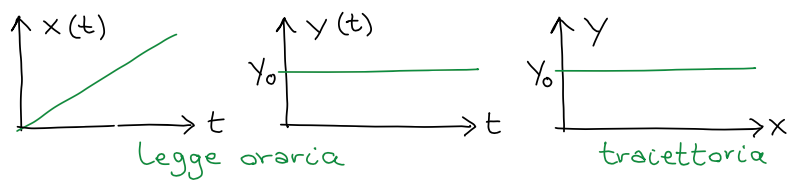
\includegraphics[width=0.8\textwidth]{images/ess-traiettoria.png}
    \end{figure}
\end{example}

\begin{definition}
    La \textbf{velocità istantanea} è la derivata della posizione rispetto al tempo.
    $$v = \lim_{\Delta t \to 0}\frac{\Delta s}{\Delta t} = \frac{ds}{dt}$$
\end{definition}

\begin{definition}
    La \textbf{velocità media} è definita come il rapporto tra lo spostamento e l'intervallo di tempo necessario per effettuarlo.
    $$v_m = \frac{\Delta s}{\Delta t}$$
\end{definition}
\hspace{-15pt}In parole povere è una grandezza che ci dice con quale rapidità cambia la posizione di un punto rispetto al tempo nell'instante $t$.
\subsection*{Vettore velocità}
Derivata rispetto al tempo del vettore posizione e si indica come 
$\frac{d\vec{r}(t)}{dt}\text{ oppure }\dot{\vec{r}}(t)[m/s]$
\begin{equation}
    \begin{split}
    \dot{\vec{r}}(t) & = (\dot{x}(t), \dot{y}(t), \dot{z}(t)) \\
     & = \frac{d}{dt}[x(t)\hat{x} + y(t)\hat{y} + z(t)\hat{z}] \\
     & = \dot{x}(t)\hat{x} + \dot{y}(t)\hat{y} + \dot{z}(t)\hat{z}
    \end{split}
\end{equation}
Per ricavare la forma esplicita uso le proprietà delle derivate (\textbf{linearità}, \textbf{Leibnitz})
\begin{example}
    $\vec{r}(t) = (v_0t, y_0, 0) = v_0t\hat{x} + y_0\hat{y}$ \:\:\:abbiamo che \:\:\:
    $\dot{\vec{r}}(t) = (v_0, 0, 0) = v_0 \hat{x}$
\end{example}
\hspace{-15pt}Velocità e spazio percorso ("integrale di linea").\\
\begin{wrapfigure}[3]{l}{5cm}
    \centering
    \includegraphics[width=5cm]{images/vettore-velocità.png}
\end{wrapfigure}
\begin{align*}
    L & = ||\vec{r}(t_1) - \vec{r}(t_0)|| + ||\vec{r}(t_2) - \vec{r}(t_1)|| + ||\vec{r}(t_3) - \vec{r}(t_2)|| + \dots \\
    & = \sum_i ||\vec{r}(t_{i+1} - \vec{r}(t_i)|| \:\: per\:\: |t_{i+1} - t_i| \text{"piccolo"} \\
    & = \sum_i ||\frac{\vec{r}(t_{i+1}) - \vec{r}(t_i)}{t_{i+1} - t_i}|| (t_{i+1} - t_i) = \int_{t_{in}}^{t_{f_{in}}}||\dot{\vec{r}}(t)||\\
\end{align*}
\begin{example}
    $\vec{r}(t) = (v_0t, y_0)\:\:\: \dot{\vec{r}}(t) = (v_0, 0)$\hspace{15pt}
    $||\dot{\vec{r}}(t)|| = \sqrt{v_0^2 + 0^2} = |v_0|$ \:\:\: $L = |v_0| \cdot (t_{f_{in}} - t_{in})$\\
    Il vettore è costante quindi facendo la derivata torna zero. Con la velocità si calcolo lo spazio percorso ("integrale di linea").
    La differenza fra le posizioni e la differenza dei tempi è il rapporto incrementale in caso gli intervalli siano sufficentemente
    piccoli, da qui si ottiene l'integrale.
\end{example}

\subsection{Vettore accelerazione}
Derivata rispetto al tempo del vettore velocità e si indica con $\frac{d^2\vec{r}(t)}{dt} \text{ oppure } \ddot{\vec{r}}(t) [m/s^2]$
\begin{equation}
    \ddot{\vec{r}}(t) = (\ddot{x}(t), \ddot{y}(t), \ddot{z}(t))\:\: = \:\: \ddot{x}(t)\hat{x} + \ddot{y}(t)\hat{y} + \ddot{z}(t)\hat{z}
\end{equation}
\begin{example}
    $\vec{r}(t)= (\frac{1}{2}a_0t^2, v_0t, 0)$ \hspace{10pt} $\dot{\vec{r}}(t) = (a_0t, v_0, 0)$ \hspace{10pt} $\dot{\vec{r}}(t) = (a_0, 0, 0)$
\end{example}
\hspace{-15pt}Serve perché l'equazione "del moto" di Newton che determinata la legge oraria è formulata in termini di accelerazione.

\subsection{Vettore quantità di moto}
Il prodotto di massa [kg] e velocità [m/s]
$$\vec{p}(t) = m \cdot \dot{\vec{r}}(t) = (m\dot{x}(t), m\dot{y}(t), m\dot{x}(t)) = m\dot{\vec{x}}(t)x + m\dot{\vec{y}}(t)y + m \dot{\vec{z}}(t)z$$
\begin{example}
    Prendiamo un punto di massa 2kg e velocità 3m/s lungo $\hat{x}$.\\
    $p_x(t) = 2 \cdot 3 kg\cdot m/s = 6 kg \cdot m/s$ \hspace{15pt} $p_y(t) = p_z(t) = 0$.
\end{example}
\hspace{-15pt}Serve per generalizzare l'equazione di Newton e per trattare sistemi di piu punti materiali.

\subsection{Vettore momento angolare rispetto a un polo P}
$$\vec{L}_p(t) = m(\vec{r}(t) - \vec{r}_p) \times \dot{\vec{r}}(t)$$
Dove $\vec{r}_p$ è il vettore posizione di p, mentre $\dot{\vec{r}}(t)$ è il prodotto vettoriale.
\begin{example}
    $\vec{r}_p = (l_0, 0, 0)$ \hspace{15pt} $\vec{r}(t) = (v_0t, y_0, 0)$\\
    $\vec{L}_p = m[(v_0t - l_0)\hat{x} + y_0\hat{y}] \times (v_0\hat{x}) \:\: = \:\: m(v_0t - l_0)v_0 \hat{x} \times \hat{x} + my_0v_0\hat{y}\times \hat{x} 
    \:\: = \:\: my_0v_0(-\hat{z}) = (0,0, -my_0v_0)$\\
    Ricorda che $\hat{x} \times \hat{x} = 0$ e $\hat{y} \times \hat{x} = -\hat{z}$
\end{example}
\hspace{-15pt}Il momento angolare dice quanta inerzia ha un oggetto in una rotazione (descrizione sommaria).\\
Il polo P è parte della definizione. È una scelta! Il risultato dipende dal polo.
Serve per formulare l'equazione del moto di sistemi di punti materiali e corpi rigidi.

\subsection{Coordinate polari}
Un metodo per rapprensentare delle cordinate x, y andando a misurare prima la distanza dall'origine e poi si va a vedere
quanto vale l'angolo fra questo segmento dall'asse x, utilizzando seno e coseno.
\begin{wrapfigure}[7]{l}{2cm}
    \centering
    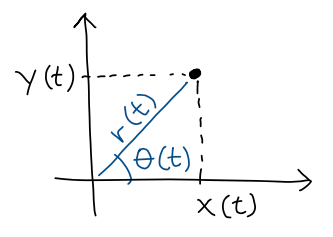
\includegraphics[width=5.5cm]{images/coordinate-polari.png}
\end{wrapfigure}
\begin{align*}
    \begin{cases}
        x(t) = r(t) \cdot \cos(\Theta(t))\\
        y(t) = r(t) \cdot \sin(\Theta(t)) 
    \end{cases}
\end{align*}
\begin{align*}
    \begin{cases}
        r(t) = \sqrt{x(t)^2 + y(t)^2} \geq 0\\
        tg(\Theta(t)) = y(t) / x(t) 
    \end{cases}
\end{align*}
\\
\begin{example} Esempi di rappresentazione di coordinate in coordinate polari.\\
    $x = 0, y = l_0 > 0 \:\: \Rightarrow \:\: r = l_0, \Theta = \pi/2$\\
    $x = 0, y = -l_0 < 0 \:\: \Rightarrow \:\: r = l_0, \Theta = -\pi/2$\\
    $x = l_0, y = l_0 > 0 \:\: \Rightarrow \:\: r = \sqrt{2}l_0, \Theta = \pi/4$\\
\end{example}

\subsection{Versori polari (2D)}
Definisco un versore $\hat{r}(t)$ che punta verso il punto materiale e un versore $\hat{\Theta}(t)$ ortogonale.
Si esprime facilmente in coordinte polari.
$$\vec{r}(t) = (x(t), y(t)) = (r(t)\cos \Theta(t), r(t)\sin\Theta(t)) \:\: = \:\: r(t)(\cos\Theta(t)\hat{x} + \sin\Theta(t)\hat{y})$$
Ma $||\vec{r}(t)|| = |r(t)| = r(t)$ allora definisco $\hat{r}(t) = \vec{r}(t)/ ||\vec{r}(t)|| = \cos \Theta(t)\hat{x} + \sin\Theta(t)\hat{y}$\\\\
Trovo facilmente che un versore ortogonale è:
$$\hat{\Theta(t)} = -\sin\Theta(t)\hat{x} + \cos\Theta(t)\hat{y} \:\:\:\text{infatti} \:\:\: \hat{r}\cdot \hat{\Theta} = c \cdot (-s) + s \cdot c = 0$$
\begin{wrapfigure}[7]{r}{6cm}
    \centering
    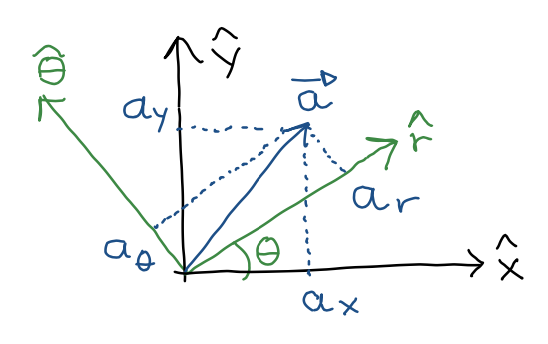
\includegraphics[width=5.5cm]{images/trasformazioni-inverse.png}
\end{wrapfigure}
\begin{note}
    Non c'è legame fra $\Theta$ e $\hat{\Theta}$ è solo una convenzione.
\end{note}
\hspace{-15pt}Le trasformazioni inverse invece si fanno come segue (verifico per sostituzione):
$$\hat{y} = \cos\Theta(t)\hat{r} - \sin\Theta(t)\hat{\Theta} \hspace{20pt} \hat{y} = \sin\Theta(t)\hat{r} + \cos\Theta(t)\hat{\Theta}$$
Possono quindi scrivere ogni vettore nella forma $\vec{a} = a_r\hat{r} + a_{\Theta}\hat{\Theta}$ con le componenti polari $a_r, a_{\Theta}$.
Per evitare ambiguità non scriviamo $(a_r, a_{\Theta})$ e riserviamo la notazione alle componenti cartesiane.\\\\
A differenza dei versori cartesiani quelli polari dipendono dal tempo per costruzioni.
$$\dot{\hat{r}}(t) = \frac{d}{dt}[\cos\Theta(t) \hat{x} + \sin\Theta(t)\hat{y}] \:\: = \:\: -\sin\Theta(t) \cdot \dot{\Theta}(t)\hat{x} + \cos\Theta(t) \cdot \dot{\Theta}(t)\hat{y}$$
Dove $\cos\Theta(t) \cdot \dot{\Theta}(t)$ si applica la derivata della somma, Leibnitz, funzione composta.
$$= \dot{\Theta}(t)\cdot \hat{\Theta}(t) \:\:\:\:(\text{confronto l'espressione di} \hat{\Theta}(t))$$
Similmente $\dot{\hat{\Theta}}(t)= - \dot{\Theta}\hat{r}(t)$.


\subsection*{Vettori posizione, velocità, accelerazione}
$$\vec{r}(t) = r(t)\hat{r}(t)$$
Dove abbiamo che $\vec{r}(t)$ è il vettore, $r(t)$ è una coordinata polare, $\hat{t}(t)$ è il versore polare.
$$\dot{\vec{r}}(r) = \dot{r}(t)\hat{r}(t) + r(t)\dot{\Theta}(t)\hat{\Theta}(t)$$
Dove la parte $\dot{\vec{r}}(r)$ è la velocità radiale.
$$\ddot{\vec{r}}(t) = [\ddot{r}(t) - r(t)\dot{\Theta}(t)^2] \hat{r} + [r(t) \ddot{\Theta}(t) + 2\dot{r}(t)\dot{\Theta}(t)]\hat{\Theta}$$
Nel quale abbiamo che la parte $r(t)\dot{\Theta}(t)^2$ si chiama \textbf{velocità centripeta}, mentre $2\dot{r}(t)\dot{\Theta}(t)$ si dice \textbf{accelerazione di Coriolis}.


	% !TeX spellcheck = it_IT
\newpage
\section{Container}
I container sono un metodo per creare la virtualizzazione e l'isolamento delle risorse in maniera più semplice.\\
La struttura è simile a quella della virtualizzazione, dove al posto dell'hypervisor abbiamo un \textbf{container manager}. La differenza principale è, però, che tutti i container operano sopra ad un unico OS, permettendo di risparmiare molte risorse sia in termini di performance che di spazio.

\subsection{Storia}
\begin{itemize}
	\item UNIX \textbf{chroot} permetteva isolamento dal filesystem
	\item FreeBSD \textbf{jail} estese l'isolamento di chroot ai processi
	\item Google inizia a sviluppare i \textbf{CGroups} per il kernel di Linux
	\item I \textbf{Linux Container} forniscono una soluzione completa
	\item \textbf{Docker} aggiunge il concetto di immagini portabili e grafica semplice da utilizzare
\end{itemize}

\subsection{Docker}
Docker è una piattaforma che permette di sviluppare ed eseguire applicazioni in un ambiente isolato sfruttando i container.\\
I componenti software sono gestiti come \textbf{immagini} in sola lettura su cui vengono creati ed eseguiti i \textbf{container}. In aggiunta possono essere montati dei \textbf{volumi} per garantire la persistenza dei dati.

\subsubsection{Images}
Sono in sola lettura e vengono salvate in un \textbf{docker registry}, pubblico o privato, strutturati in repositories che contengono ognuna ogni versione di un determinato software.

\subsubsection{Swarm mode}
Docker prevede la \textbf{swarm mode} per gestire un gruppo di container (swarm). I \textbf{nodi} possono essere:
\begin{itemize}
	\item \emph{Managers}, che delegano le task ai workers
	\item \emph{Workers}, che eseguono le task a loro assegnate
\end{itemize}
L'utente può definire lo stato desiderato dei vari servizi dell'applicazione. Ogni nodo avrà un DNS name univoco. Swarm si occuperà di fare \emph{load balancing} e di mantenere la coerenza degli stati secondo quello desiderato.
	% !TeX spellcheck = it_IT
\newpage
\section{FaaS}
L'approccio FaaS è un mercato in crescita e ad oggi esistono molteplici opzioni tra le quali scegliere. In particolare le suddividiamo in due categorie: \emph{commerciali} (e.g. AWS Lambda) e \emph{open source} (e.g. Apache Openwisk).\\
Per fare una scelta consapevole, dobbiamo analizzare le proposte da due punti di vista: quello commerciale e quello tecnico.
\subsection{Business view}
\subsubsection{Licensing}
Tutte le piattaforme \textbf{open source} usano licenze abbastanza permissive, come ad esempio Apache 2.0. Quelle \textbf{commerciali} invece usano software proprietario, fatta eccezione per MS Azure Functions che ha alcune componenti libere.
\begin{center}
	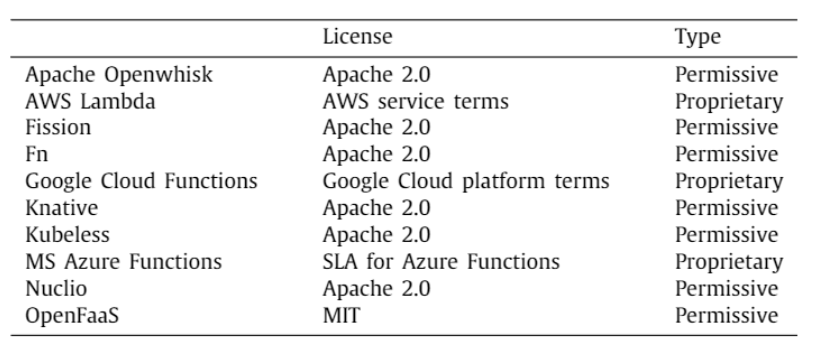
\includegraphics[scale=0.4]{faas_licensing.png}
\end{center}
\subsubsection{Installazione}
Tra le opzioni commerciali solamente Azure functions ha dei servizi installabili \emph{on-premises}. Quelle open source supportano invece molteplici host, con Kubernetes tra i più popolari.
\begin{center}
	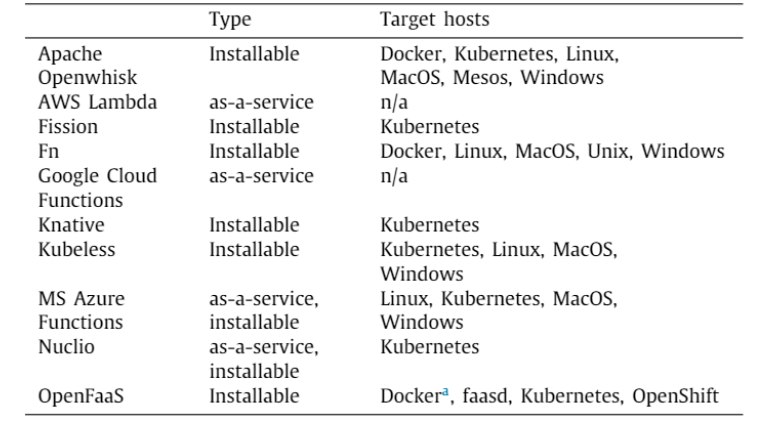
\includegraphics[scale=0.4]{faas_installation.png}
\end{center}
\newpage
\subsubsection{Source code}
Tutte le piattaforme open source sono hostate su GitHub ed implementate in Go.
\begin{center}
	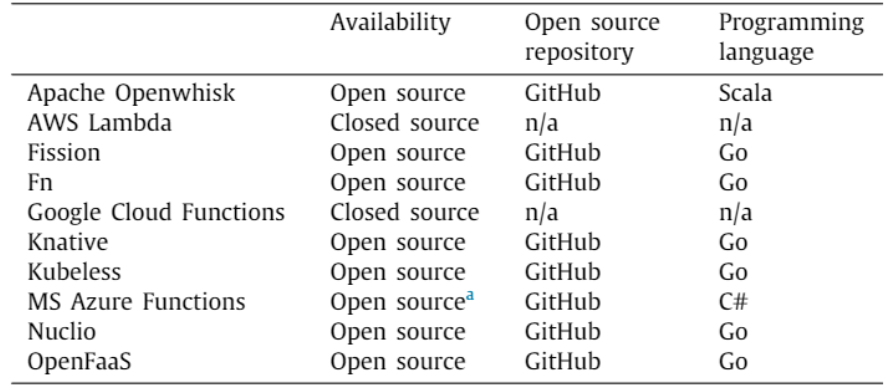
\includegraphics[scale=0.4]{faas_opensource.png}
\end{center}
\subsubsection{Interfaccia}
Tutte le piattaforme forniscono CLI, mentre API e GUI  non sono sempre presenti in quelle open source. Inoltre in queste ultime il metodo di amministrazione cambia molto tra l'una e l'altra.
\begin{center}
	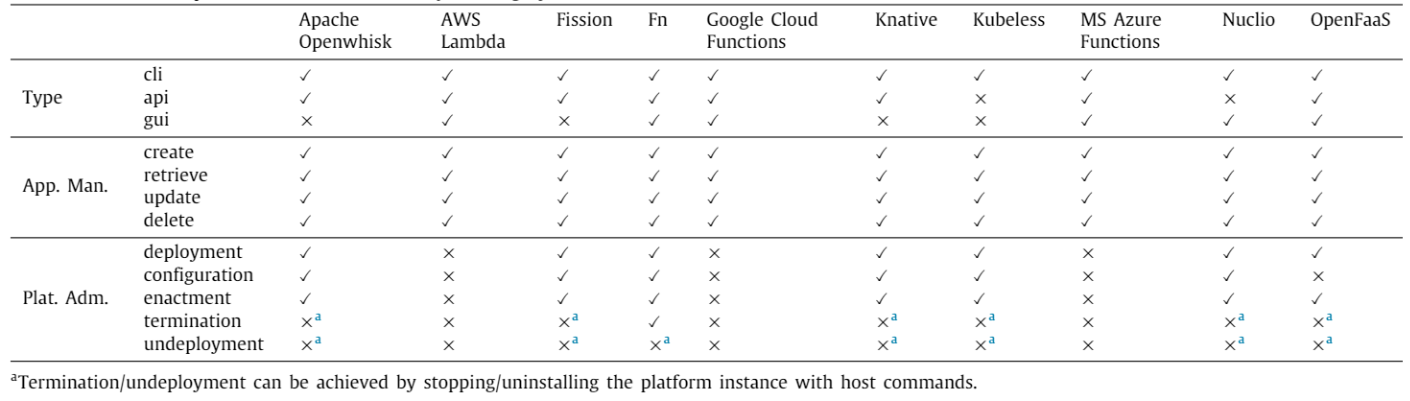
\includegraphics[scale=0.3]{faas_interface.png}
\end{center}
\subsubsection{Community}
Le piattaforme open source sono molto ben votate su GitHub ma poco cercate e diffuse su StackOverflow, a differenza di quelle commerciali.
\begin{center}
	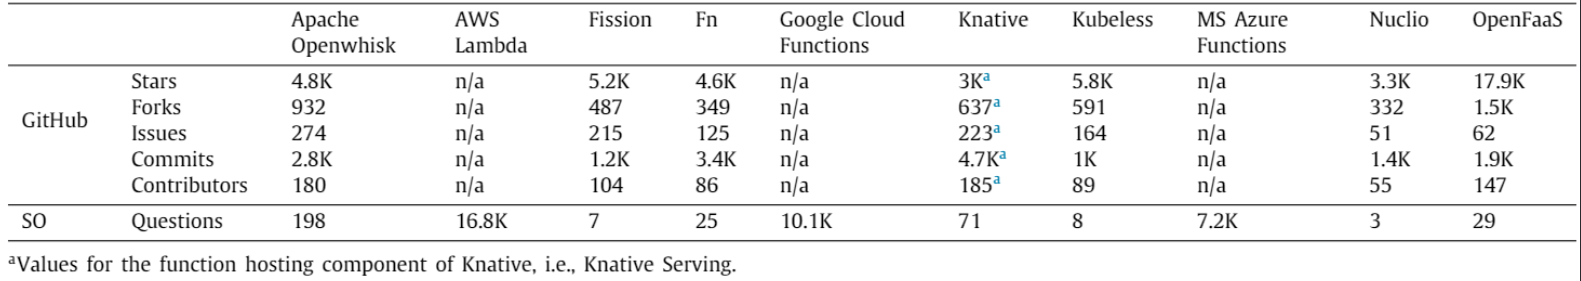
\includegraphics[scale=0.3]{faas_community.png}
\end{center}
\subsubsection{Documentazione}
Tutte le piattaforme forniscono la documentazione per l'utilizzo e il deploy del servizio ma non tutte le loro architetture sono documentate.
\begin{center}
	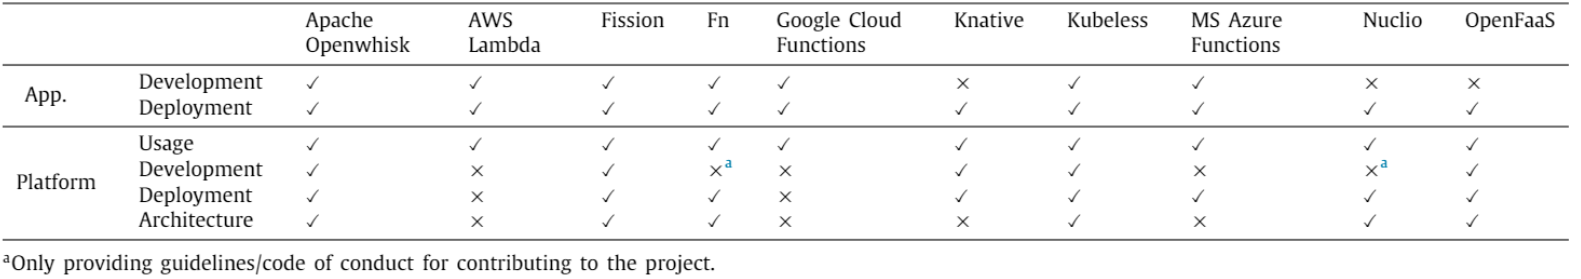
\includegraphics[scale=0.25]{faas_documentation.png}
\end{center}
\subsection{Technical view}
\subsubsection{Sviluppo}
I linguaggi più comuni nello sviluppo in ambito FaaS sono Java, NodeJS e Python, con il supporto di Docker.
\begin{center}
	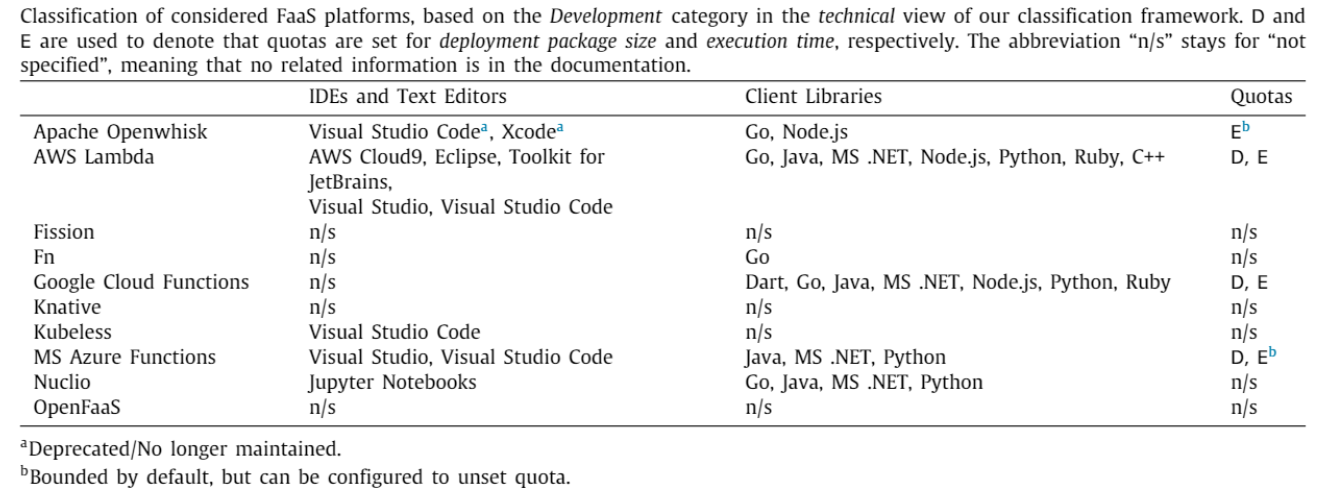
\includegraphics[scale=0.33]{faas_developement.png}
\end{center}
\subsubsection{Versioning}
La maggior parte delle piattaforme implementano un sistema di versioning in maniera implicita, al contrario di quelle commerciali:
\begin{itemize}
	\item \textbf{Dedicated mechanisms}
	\item \textbf{Implicit mechanisms}
\end{itemize}
\begin{center}
	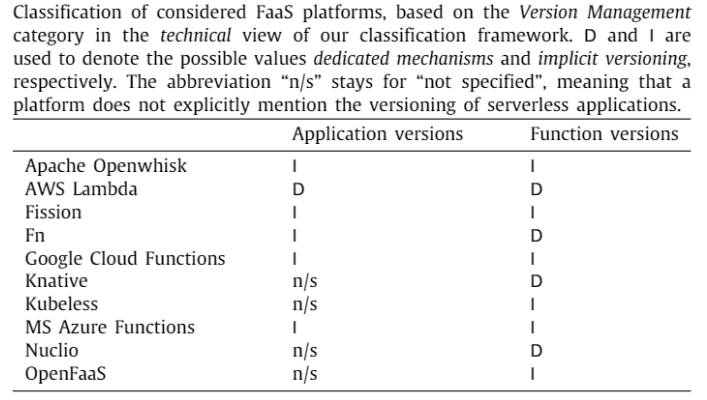
\includegraphics[scale=0.4]{faas_versioning.png}
\end{center}
\subsubsection{Event sources}
Tutte le piattaforme supportano la chiamata di funzioni tramite richieste \textbf{sincrone} HTTP, mentre solo alcune supportano quelle \textbf{asincrone}. Più della metà non supportano il salvataggio dei \textbf{dati delle richieste}. Gli \textbf{scheduler}, gli \textbf{stream processing} e il \textbf{messaging} sono ampiamente supportati. Più della metà delle piattaforme documentano la possibilità di creare \textbf{eventi personalizzati}.
\newpage
\subsubsection{Function orchestration}
Più della metà delle piattaforme supportano il function orchestration tramite DSL proprietari o funzioni apposite.
\begin{center}
	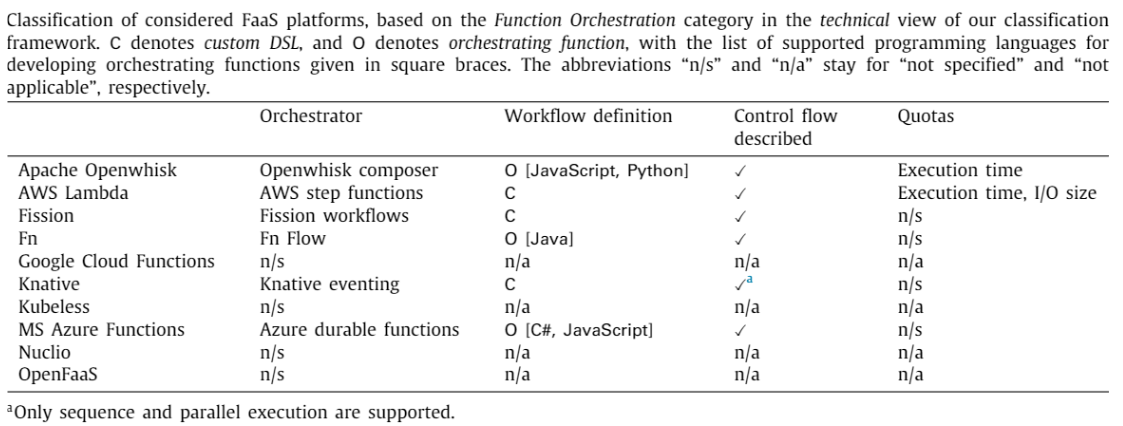
\includegraphics[scale=0.38]{faas_orchestration.png}
\end{center}

\subsubsection{Testing e debugging}
La maggior pare delle piattaforme supporta testing funzionale e debugging delle funzioni. La differenza sta nella sofisticatezza di questi sistemi, che è più elevata per le piattaforme commerciali.
\subsubsection{Logging}
Le piattaforme commerciali usano strumenti ad hoc per monitorare lo stato del servizio mentre quelle open source si rifanno a servizi terzi.
\begin{center}
	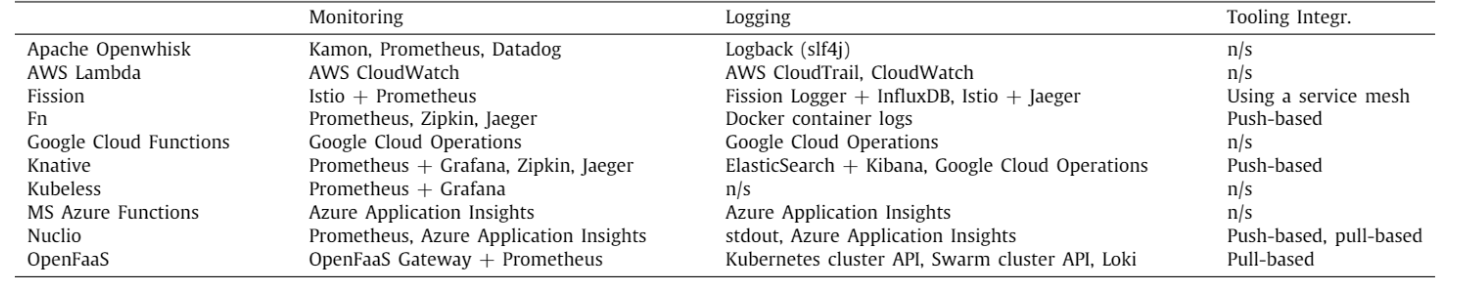
\includegraphics[scale=0.3]{faas_logging.png}
\end{center}
\subsubsection{Application delivery}
La maggior parte delle piattaforme segue un approccio dichiarativo per automatizzare il deploy delle applicazioni. Solo quelle commerciali supportano la pipeline di tipo CI/CD (Continuous Implementation/Continuous Deployment).
\begin{center}
	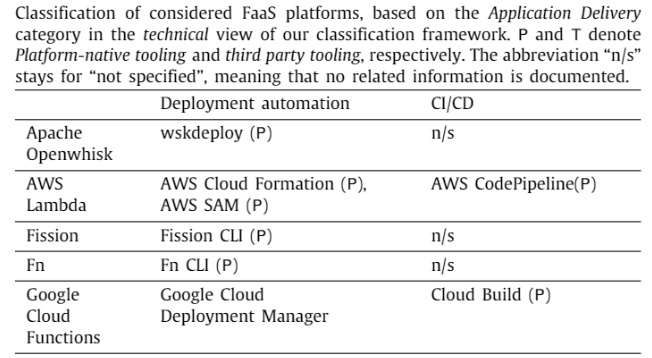
\includegraphics[scale=0.3]{faas_deployment_1.png}
	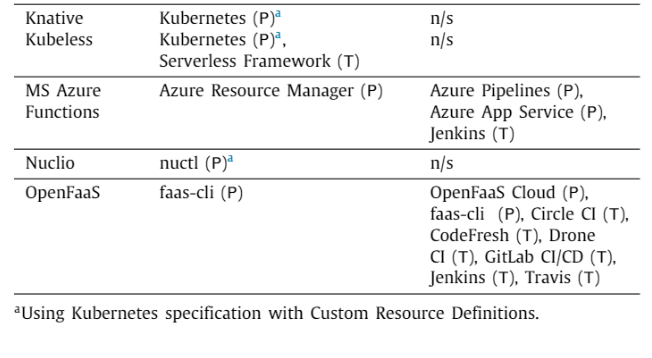
\includegraphics[scale=0.3]{faas_deployment_2.png}
\end{center}
\subsubsection{Riuso}
Solamente AWS Lambda e MS Azure Functions prevedono un marketplace per condividere e riutilizzare funzioni.
\subsubsection{Gestione degli accessi}
Le piattaforme commerciali supportano nativamente l'autenticazione e il controllo delle risorse. Quelle open source di solito sfruttano features del sistema operativo.

	% !TeX spellcheck = it_IT
\newpage
\section{PaaS}
L'approccio PaaS prevede che i fornitori esterni gestiscano sia hardware che software e che l'utente fornisca solamente i dati e l'applicativo.\\
I \textbf{vantaggi} sono:
\begin{itemize}
	\item Ridotta gestione per l'utente
	\item Manutenzione automatica
	\item Load balancing, scaling e distribuzione più efficienti
	\item Più facilità nell'adottare nuove tecnologie
\end{itemize}
Gli \textbf{svantaggi} invece:
\begin{itemize} 
	\item Disponibilità del servizio molto dipendente dal fornitore
	\item Vendor lock-in
	\item In balia di eventuali cambiamenti da parte del fornitore
\end{itemize}
\subsection{Heroku}
Heroku è una piattaforma cloud basata sulla gestione di un sistema di container, con data services integrati e un ampio ecosistema, per sviluppare ed eseguire app moderne.\\
Gli utenti usano \textit{container} chiamati \textbf{dynos} per lanciare ed eventualmente scalare le loro applicazioni. Questi sono container linux virtualizzati ed isolati progettati per eseguire codice 
	% !TeX spellcheck = it_IT
\newpage
\section{Business models}
Il \textbf{business model} descrive l'idea di come un'organizzazione crea, consegna e cattura del \textbf{valore}.
\subsection{Canvas}
Il Business Model Canvas è un linguaggio condiviso per descrivere, visualizzare, valutare e modificare modelli di business. Si struttura come segue:
\begin{center}
	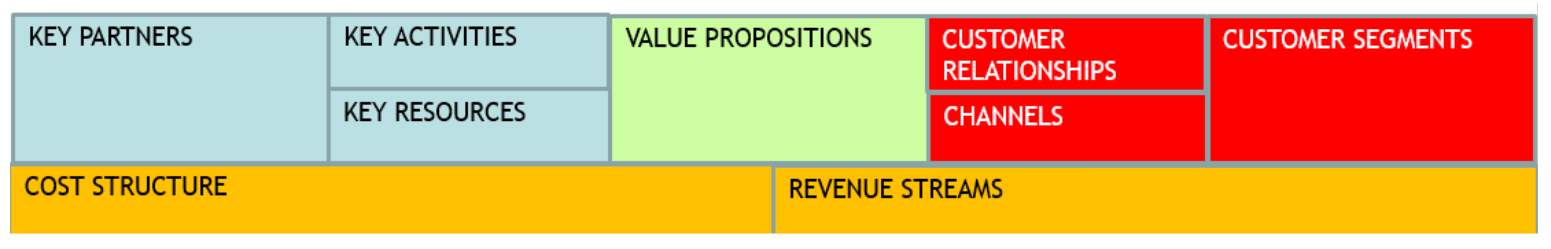
\includegraphics[scale=0.25]{business_model_canvas.png}
\end{center}
Vediamo nel dettaglio ogni sezione:
\begin{itemize}
	\item \textbf{Value propositions}: descrive l'insieme di prodotti e servizi che creano valore per un segmento specifico di clienti
	\item \textbf{Customer}
	\begin{itemize}
		\item \textbf{Segments}: definisce i diversi gruppi di persone o organizzazioni che un'impresa vuole raggiungere e servire
		\item \textbf{Relationship}: descrive i tipi di relazioni che un'azienda stabilisce con determinati segmenti
		\item \textbf{Channels}: descrive come l'azienda comunica e raggiunge i segmenti
	\end{itemize}
	\item \textbf{Key}
	\begin{itemize}
		\item \textbf{Resources}: le risorse più importanti per far funzionare un business model
		\item \textbf{Activities}: le attività più importanti per far funzionare un business model
		\item \textbf{Partners}: la rete di fornitori e partner che fanno funzionare un business model
	\end{itemize}
	\item \textbf{Revenue streams}: il guadagno di un'azienda diviso per ogni segmento
	\item \textbf{Cost structure}: tutti i costi strutturali previsti dal business model
\end{itemize}

\begin{example}[Nespresso]
	Nel 1976 la \textit{Nestré} dominava il mercato con il caffè istantaneo tramite il prodotto Nescafé. \\
	Nel 1988 la Nespresso riesce a ribaltare la situazione concentrandosi su segmenti di mercato di elite. In particolare, usa il seguente canvas:
	\begin{center}
		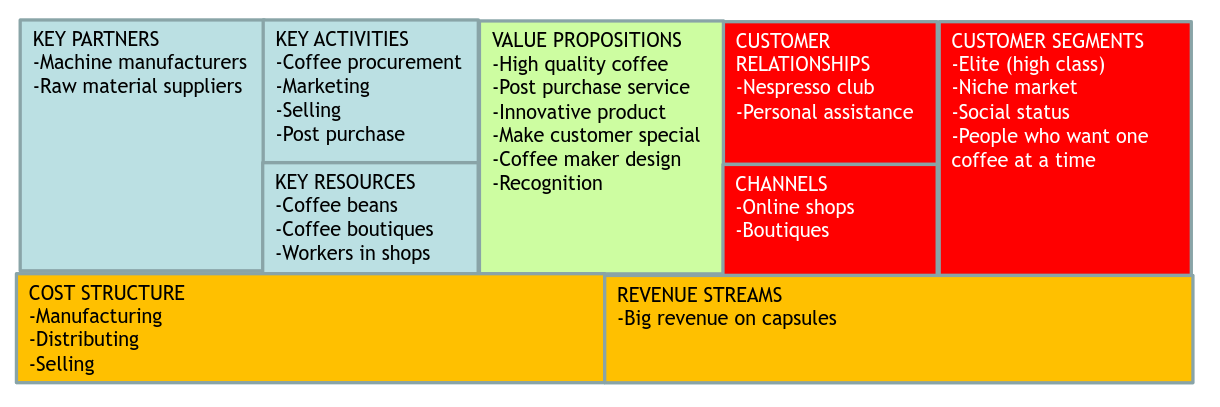
\includegraphics[scale=0.35]{nespresso_canvas.png}
	\end{center}
\end{example}

\newpage
\begin{example}[Netflix]
	Netflix è riuscito a spodestare il dominio di aziende come Blockbuster introducendo lo streaming. Vediamo il confronto tra i due canvas:
	\begin{center}
		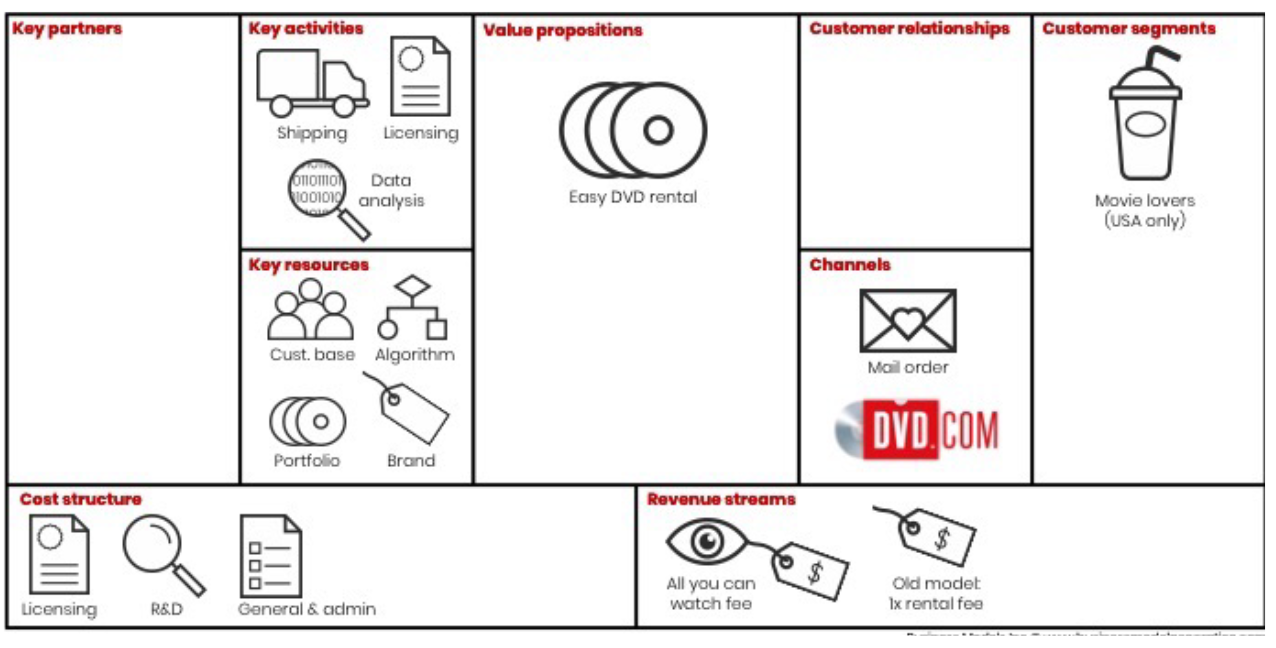
\includegraphics[scale=0.17]{blockbuster.png}
		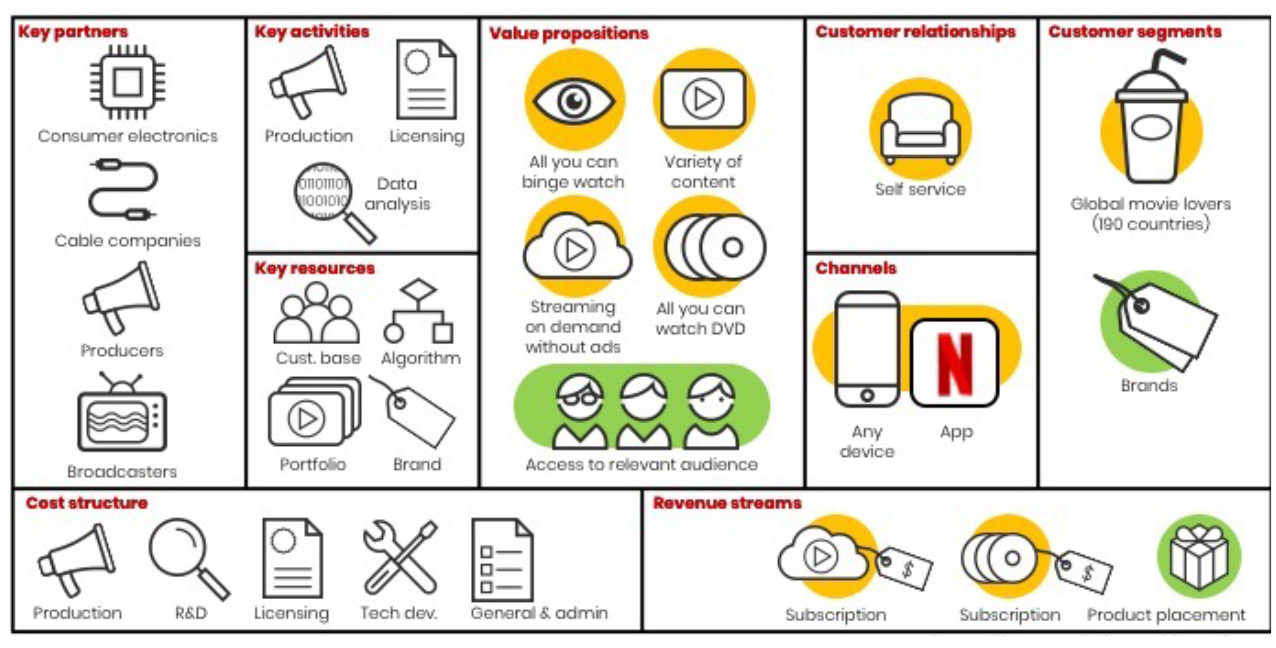
\includegraphics[scale=0.17]{netflix.png}
	\end{center}
\end{example}

\subsection{Freemium}
L'idea è di combinare funzionalità di base gratuite con servizi più avanzati a pagamento, tenendo d'occhio quanto costa all'azienda mantenere i servizi gratuiti e a che rateo gli utenti diventano premium.\\
In media il $10\%$ di tutti gli utenti diventano premium.

\begin{example}[Spotify]
	Spotify ha gli utenti gratuiti che fanno guadagnare tramite le pubblicità e quelli a pagamento che pagano l'abbonamento. Spotify deve poi pagare le commissioni a chi detiene i diritti sulla musica.
	\begin{center}
		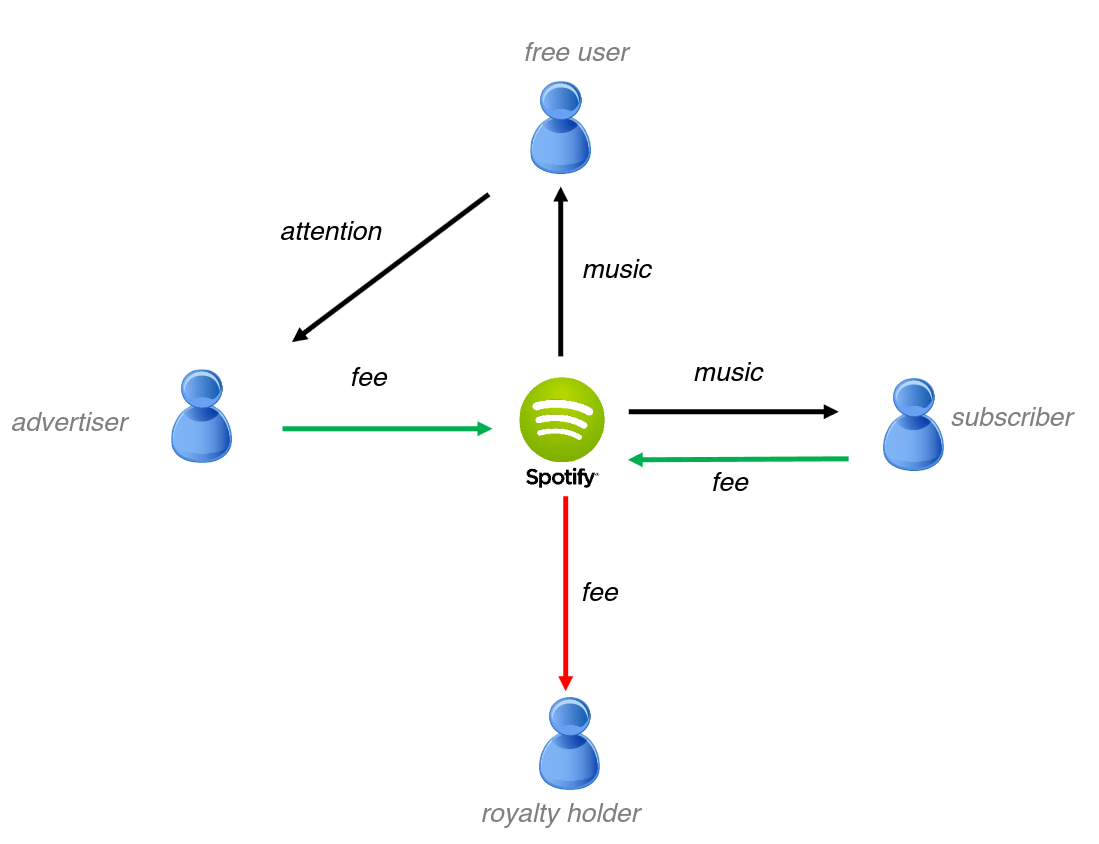
\includegraphics[scale=0.3]{spotify.png}
	\end{center}
\end{example}
\newpage
\begin{example}[Flickr]
	Vediamo il canvas di Flickr:
	\begin{center}
		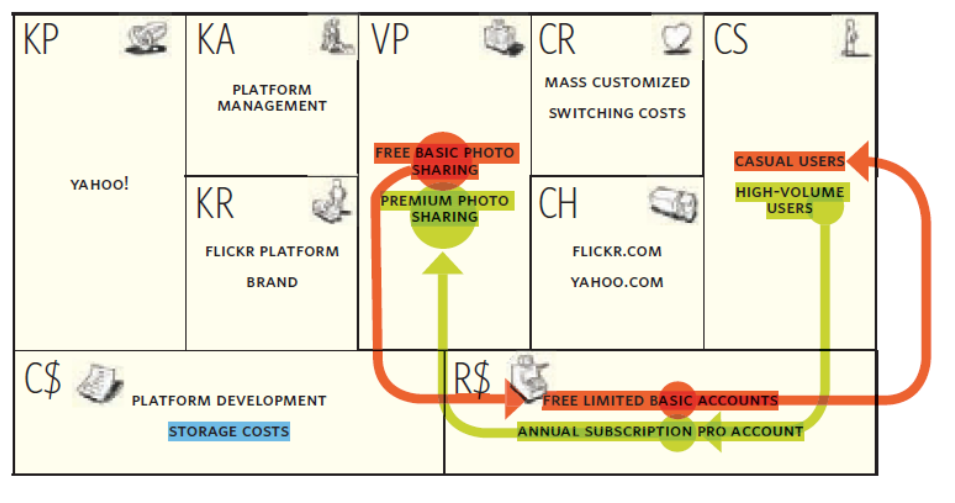
\includegraphics[scale=0.3]{flickr.png}
	\end{center}
	Anche Flickr si basa su un principio \textit{freemium}: in \color{red}rosso \color{black} il tier gratuito mentre in \color{green}verde \color{black} quello a pagamento.
\end{example}

\begin{example}[Redhat]
	Redhat si concentra sul segmento di mercato delle aziende che vogliono sfruttare prodotti opensource ma che vogliono anche che ci sia qualcuno di responsabile (anche legalmente).
	\begin{center}
		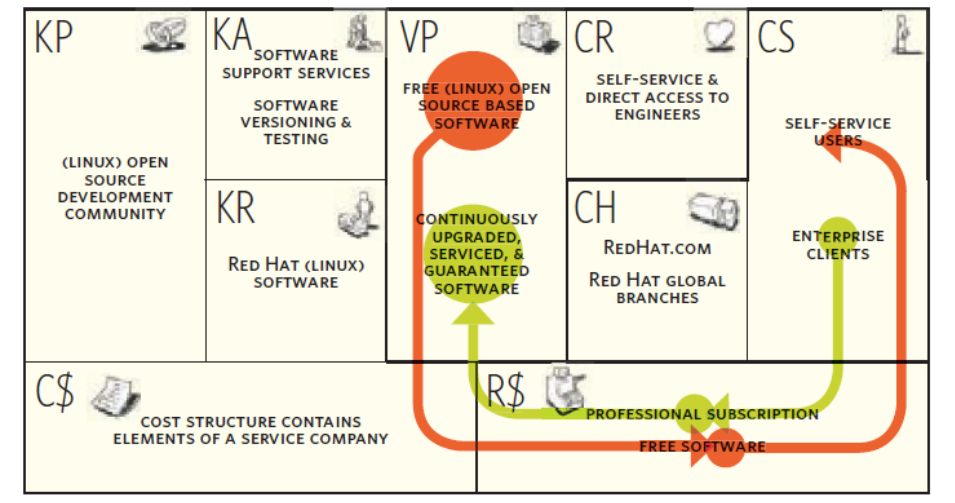
\includegraphics[scale=0.3]{redhat.png}
	\end{center}
\end{example}

\begin{example}[Skype]
	Permette di fare chiamate gratuite attraverso internet.
	\begin{center}
		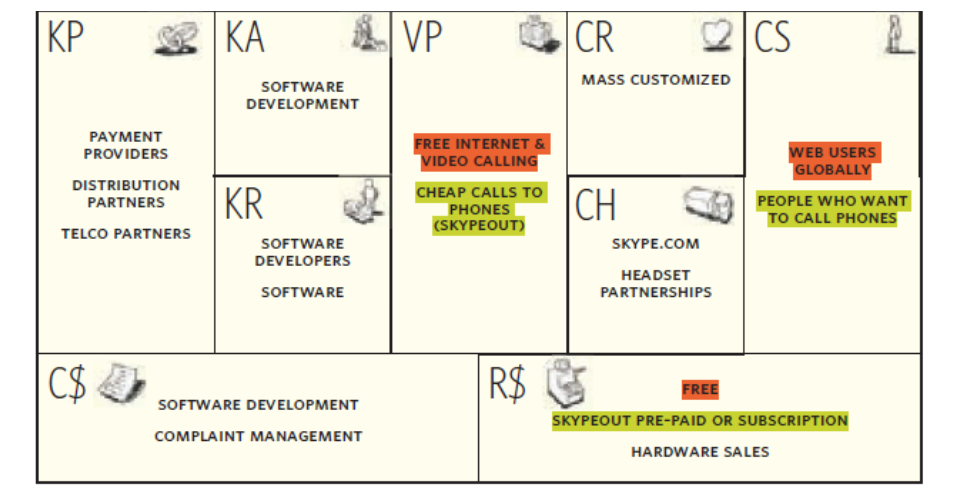
\includegraphics[scale=0.3]{skype.png}
	\end{center}
\end{example}

\begin{note}
	Anche Dropbox utilizza un principio freemium. A differenza di Netflix, Dropbox si è poi distaccato da Amazon AWS e ha creato la sua infrastruttura.
\end{note}

\newpage
\subsection{Innovazione}
L'innovazione parte dal cambio di prospettiva: bisogna concentrarsi su quella del cliente. Da qui poi possiamo farci le domande \textbf{what if...?}, che ci portano ad identificare principalmente quattro epicentri di miglioramento:
\begin{itemize}
	\item \textbf{Resource Driven}: queste innovazioni nascono da un'infrastruttura preesistente per \textit{espandere} o \textit{trasformare} il business model. Un esempio è Amazon AWS.
	\item \textbf{Customer Driven}: queste innovazioni si basano sulle \textit{necessità del cliente}, sulla \textit{facilità di accesso} o sul migliorare la \textit{comodità}. Influenza delle parti specifiche del business model. Un esempio è 23andMe che offre test del DNA specifici per certe richieste.
	\item \textbf{Offer Driven}: le innovazioni di questo tipo creano una nuova \textit{value proposition}, ad esempio Cemex consegna il cemento in 4 ore invece che 48.
	\item \textbf{Finance Driven}: innovazioni che \textit{riducono i costi} o \textit{aumentano i guadagni} (anche introducendo nuove fonti). Un esempio è Xerox che fornisce le prime 2000 copie gratuite.
\end{itemize}

\subsection{Casi di studio}
\subsubsection{Amazon}
Amazon (originariamente \textit{Cadabra}) viene fondata da Jeff Bezos nel 1994 come negozio online di libri. Non si aspettava di avere profitti per i primi 4 o 5 anni e infatti il primo quadrimestre positivo è stato l'ultimo del 2001.\\
Al 2022 i guadagni (in miliardi di dollari) si dividono in:
\begin{enumerate}
	\item $231.87$ dallo store online
	\item $140.05$ dai servizi ai venditori di terze parti
	\item $90.76$ da AWS
	\item $40.20$ da abbonamenti (e.g. Prime)
	\item $20.03$ da negozi fisici
\end{enumerate}
\subsubsection{Google}
I guadagni di Google si concentrano sulle \textbf{pubblicità personalizzate}:
\begin{center}
	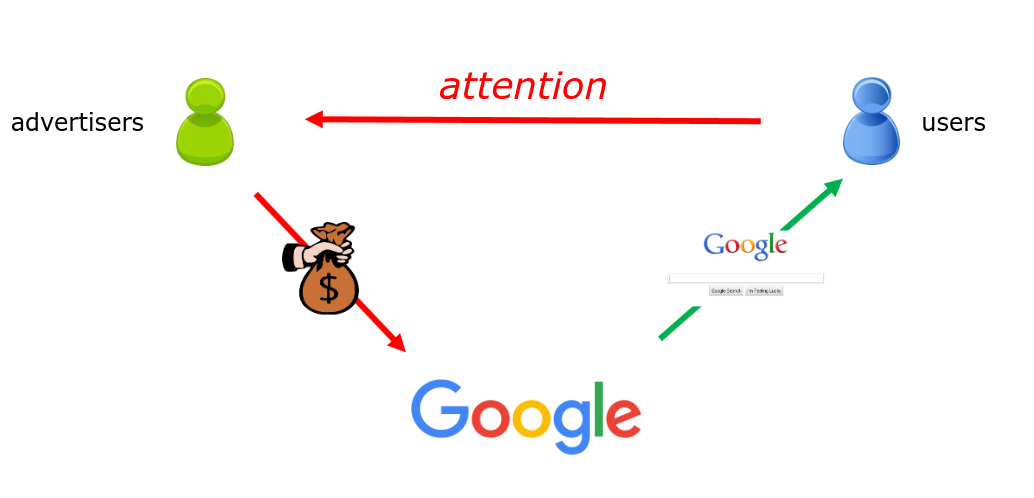
\includegraphics[scale=0.3]{google.png}
\end{center}
non solo tramite il motore di ricerca ma anche con tutte le altre applicazioni che forniscono.
	% !TeX spellcheck = it_IT
\newpage
\section{Software services}
\subsection{REST}
REST (REpresentational State Trasfer) è uno stile architetturale sviluppato come modello astratto per il Web.\\
Ogni azione causa il passaggio dell'applicazione allo stato successivo tramite il trasferimento dello stato corrente.\\
Si basa sui seguenti principi:
\begin{itemize}
	\item \textbf{URIs (Uniform Resource Identifier)}: identificazione delle risorse in maniera \textit{univoca} e \textit{universale}, ad esempio gli indirizzi Web
	\item \textbf{Interfaccia uniforme}: ad esempio per il protocollo HTTP, l'utente invoca dei metodi predefiniti:
	\begin{itemize}
		\item \textit{POST} e \textit{PUT} per creare e aggiornare risorse
		\item \textit{DELETE} per eliminare una risorsa
		\item \textit{GET} per ottenere lo stato corrente di una risorsa
	\end{itemize}
	\item \textbf{Messaggi autoesplicativi}: ogni richiesta contiene abbastanza \textit{contesto} per riuscire a comprendere il messaggio. Inoltre le risorse sono \textit{separate} dalla loro rappresentazione in modo da poter essere accedute in diversi formati
	\item \textbf{Interazioni stateful tramite hyperlinks}: data la natura stateless, per fornire interazioni stateful si utilizzano trasferimenti espliciti di stato tramite hyperlinks
\end{itemize}
\subsubsection{Negoziazione}
Quando viene richiesta una risorsa, vanno specificati i formati accettabili. Il server poi risponde con la risorsa nel formato più appropriato o eventualmente con il codice di errore 406.
\begin{center}
	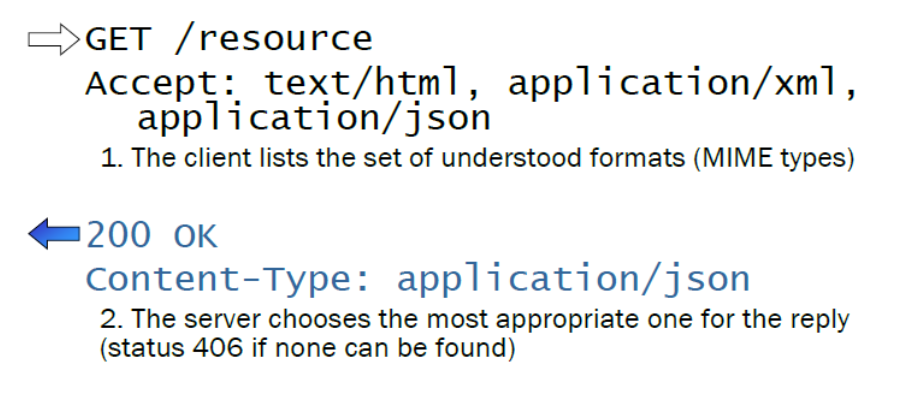
\includegraphics[scale=0.2]{negotiation.png}
\end{center}
\subsubsection{Design}
Il design deve seguire i seguenti passaggi:
\begin{enumerate}
	\item Identificare le risorse che devono essere esposte come servizi
	\item Modellare le relazioni tra le risorse tramite gli \textit{hyperlinks}
	\item Definire gli URIs seguendo le seguenti guidelines:
	\begin{itemize}
		\item Meglio i sostantivi dei verbi
		\item Brevità
		\item Utilizzare i template per costruire ed elaborare URIs parametrici
		\item Non cambiarli, nel caso utilizzare il reindirizzamento
	\end{itemize}
	\item Definire quali metodi sono applicabili alla risorsa
	\item Progettare e documentare la rappresentazione delle risorse
	\item Implementare e rilasciare il servizio
	\item Testing
\end{enumerate}
\subsubsection{Riepilogo}
L'architettura REST è \textbf{semplice} (utilizza standard famosi e infrastruttura già presente), \textbf{leggera} (sia per i protocolli utilizzati che per i messaggi) e \textbf{scalabile}. Di contro però i client possono richiedere troppi o troppi pochi dati, possono fare un numero limitato di richieste e le convenzioni per la nomenclatura sono inconsistenti.
	% !TeX spellcheck = it_IT
\newpage
\section{Kubernetes}
Kubernetes è un \textbf{orchestratore} di container. In pratica si assicura che gruppi di container che devono lavorare assieme lo facciano in maniera corretta ed efficiente (un po' come il direttore d'orchestra dà le istruzioni ai musicisti).\\
Si occupa dell'intero \textbf{ciclo di vita} del container, dall'\textit{allocazione} di risorse allo \textit{spegnimento}, nonché della \textit{comunicazione} tra container e della \textit{schedule} ottimale per completare un lavoro.
\subsection{Funzionamento}
La struttura di un sistema con Kubernetes si compone di un \textbf{orchestratore} che espone delle \textbf{API} e che è connesso con molteplici \textbf{worker}, ognuno dei quali è un container a sé stante con un \textbf{kubelet}, ovvero un processo che si occupa di comunicare con l'esterno l'orchestratore.\\
All'orchestratore viene data in pasto una configurazione che rappresenta lo \textbf{stato desiderato}, e lui poi farà in modo, con le risorse che possiede, di mantenerla sempre attiva. Questa configurazione contiene principalmente:
\begin{itemize}
	\item \textbf{Deployment}
	\item \textbf{Pod}: unità più piccola che può contenere una o più immagini di container e della quale si deve specificare il numero di istanze necessarie
\end{itemize}
Nel momento in cui un worker smette di funzionare, l'orchestratore sposta i pod che vi erano in esecuzione su un altro worker, in modo da mantenere costante il numero di repliche attive.
\subsection{Principi}
\subsubsection{Dichiaratività}
Dichiariamo lo \textbf{stato desiderato} del sistema e lasciamo che Kubernetes si occupi di fare tutto ciò che è necessario per raggiungere quell'obiettivo e risolvere eventuali problemi che possono presentarsi.\\
Lo stato desiderato lo definiamo tramite degli \textbf{oggetti}, ognuno con delle specifiche che forniscono lo stato desiderato e lo stato attuale. Kubernetes si occupa poi di verificare costantemente che lo stato attuale sia equivalente a quello desiderato e, in caso non lo sia, provare a ripararlo o sostituirlo direttamente con uno nuovo.
\subsubsection{Distribuzione}
Kubernetes fornisce un'interfaccia unificata per interagire con un cluster di macchine, evitandoci di doverci preoccupare della comunicazione con le singole.
\begin{center}
	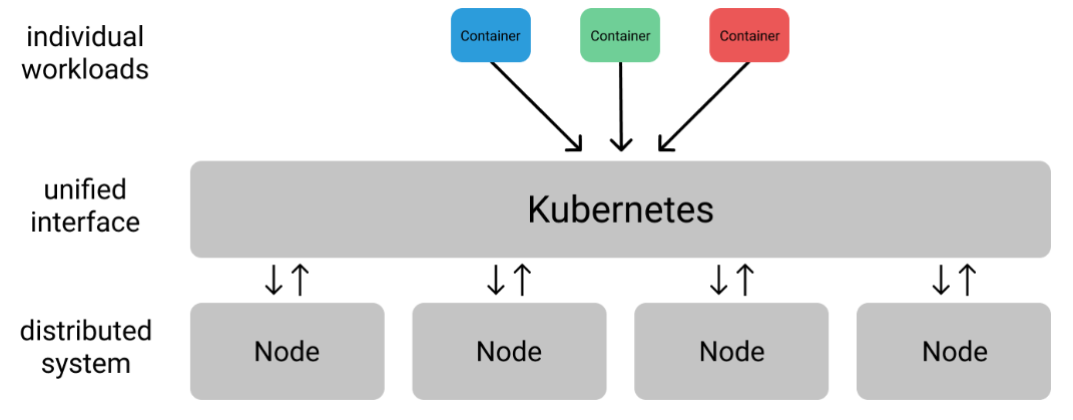
\includegraphics[scale=0.3]{kubernetes_distribution.png}
\end{center}
\subsubsection{Decoupling}
I container devono essere sviluppati in modo che abbiano un singolo compito da svolgere, seguendo i principi dei \textbf{microservizi}.
\subsubsection{Infrastruttura immutabile}
Per ottenere i maggiori benefici dall'orchestrazione di container dobbiamo lavorare basandoci sul principio di un'infrastruttura immutabile. Ad esempio invece di aggiornare eventuali librerie di un container, distruggerlo e ricrearlo da zero con gli aggiornamenti già pronti.\\
Di conseguenza durante l'intero ciclo di vita di un container dobbiamo utilizzare la stessa configurazione ed eventualmente sostituirli con nuovi. \\
Tutto questo ci permette di rendere molto semplice il rollback ad una vecchia versione.
\subsection{Oggetti}
Esistono molti oggetti in Kubernetes, noi ne vedremo solo i principali.
\subsubsection{Manifesto}
Il \textbf{manifesto} contiene la definizione degli oggetti di Kubernetes ed è scritto in \textit{YAML} o \textit{JSON}. Ogni oggetto ha le seguenti informazioni:
\begin{itemize}
	\item Che \textbf{API} usa e quale versione
	\item Che \textbf{tipo} di oggetto è
	\item Cosa \textbf{identifica} in maniera univoca l'oggetto
	\item Lo \textbf{stato} che deve avere l'oggetto
\end{itemize}

\subsubsection{Pod}
Un \textbf{pod} consiste in un insieme di uno o più \textit{container}, un livello \textbf{network} condiviso e volumi del \textbf{filesystem} condivisi.
\subsubsection{Deployment}
Un oggetto di tipo \textbf{deployment} contiene una raccolta di \textit{Pod} definiti da un template e il numero di \textbf{repliche} necessarie per ognuno di essi. Il cluster cercherà in ogni modo di mantenere attive le $n$ repliche indicate del template.
\begin{lstlisting}[style=yaml]
	apiVersion: apps/v1
	kind: Deployment
	metadata:
		name: ml-model-serving
		labels:
			app: ml-model
	spec:
		replicas: 10
		selector:
			matchLabels:
				app: ml-model
		template:
			metadata:
				labels:
					app: ml-model
			spec:
				containers:
				-  name: ml-rest-server
					image: ml-serving:1.0
					ports:
					-  containerPort: 80
\end{lstlisting}
\newpage
\subsubsection{Service}
Ogni \textit{pod} ha un indirizzo IP assegnato che viene usato per la comunicazione. Data la volatilità dei pod, che possono cessare di esistere o essere sostituiti velocemente, l'oggetto \textbf{service} fa il lavoro sporco del capire chi contattare, esponendo all'utente solo degli \textit{endpoint}. Per farlo si basa sulle \textbf{labels}.
\begin{lstlisting}[style=yaml]
	apiVersion: v1
	kind: Service
	metadata:
		name: ml-model-svc
		labels:
			app: ml-model
	spec:
		type: ClusterIP
		selector:
			app: ml-model
		ports:
		-  protocol: TCP
			port: 80
\end{lstlisting}

\subsubsection{Ingress}
Se \textit{Service} permette la comunicazione tramite un unico endpoint nella traffico locale, \textbf{ingress} permette la comunicazione con l'esterno.
\begin{lstlisting}[style=yaml]
	apiVersion: networking.k8s.io/v1beta1
	kind: Ingress
	metadata:
		name: ml-product-ingress
		annotations:
			kubernetes.io/ingress.class: "nginx"
			nginx.ingress.kubernetes.io/rewrite-target: /
	spec:
		rules:
		-  http:
				paths:
				-  path: /app
					backend:
						serviceName: user-interface-svc
						servicePort: 80
\end{lstlisting}
\newpage
\subsection{Control plane}
In un sistema di Kubernetes abbiamo due tipi di macchine:
\begin{itemize}
	\item \textbf{Master node}: spesso singola, contiene la maggior parte dei componenti del pannello di controllo
	\item \textbf{Worker node}: macchina che esegue i workflow dell'applicazione
\end{itemize}

\subsubsection{Master node}
Si compone di:
\begin{itemize}
	\item Il \textbf{server API} convalida la richiesta e fornisce le informazioni sullo stato del cluster, che è salvato in uno storage distribuito di tipo chiave-valore chiamato \textbf{ectd}.\\
	Lo stato contiene diverse informazioni tra cui la configurazione attuale, le specifiche degli oggetti, i loro stati, i nodi presenti e che lavori hanno assegnati.
	\begin{center}
		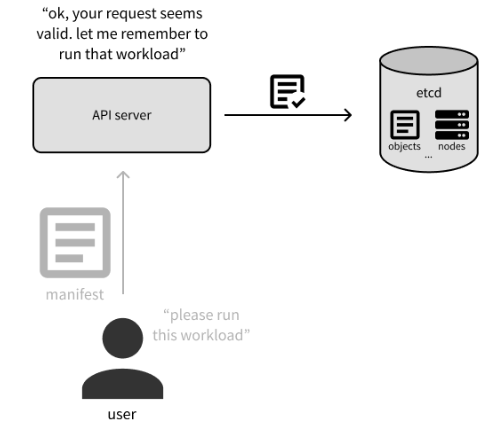
\includegraphics[scale=0.3]{api_server.png}
	\end{center}
	\item Lo \textbf{scheduler} si occupa di decidere su che nodo far partire un determinato workload richiesto:
	\begin{enumerate}
		\item Chiede al \textit{server API} quali oggetti non sono stati assegnati a delle macchine
		\item Determina a quali macchine dovrebbero essere assegnati
		\item Risponde al \textit{server API} comunicandogli gli assegnamenti eseguiti
	\end{enumerate}
	\begin{center}
		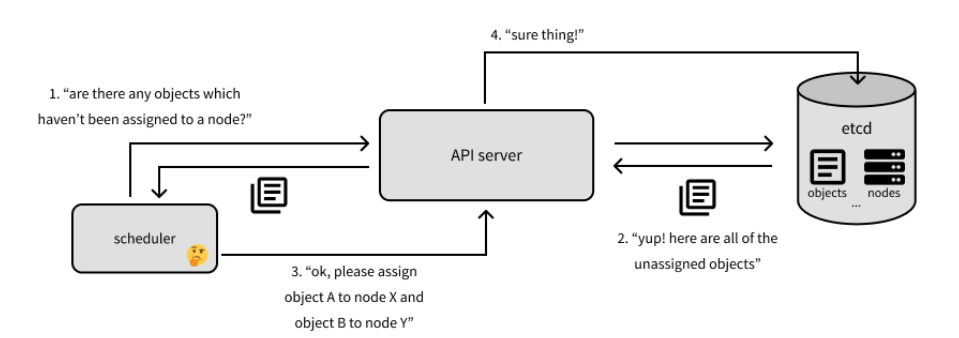
\includegraphics[scale=0.3]{scheduler.png}
	\end{center}
	\item Il \textbf{controller manager} monitora lo stato del cluster attraverso il \textit{server API}. Se lo stato attuale non è quello desiderato, esegue richieste al server in modo da farlo convergere a quello voluto
	\begin{center}
		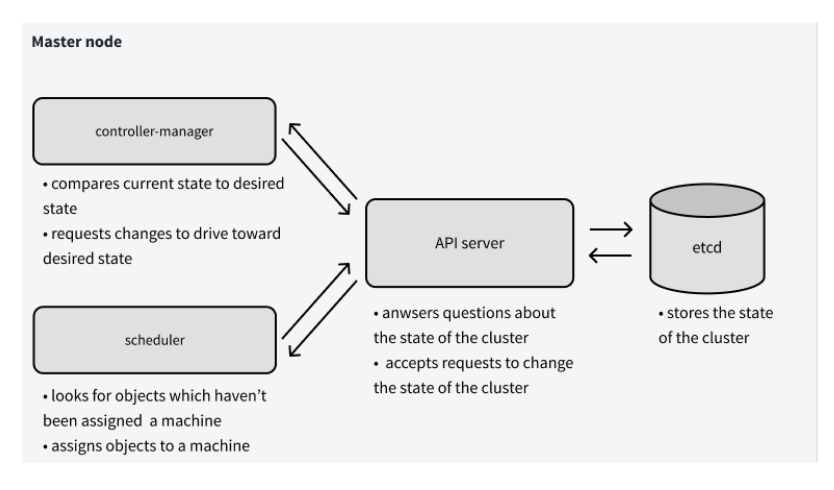
\includegraphics[scale=0.3]{controller_manager.png}
	\end{center}
\end{itemize}
\subsubsection{Worker node}
Il worker node si compone di due elementi:
\begin{itemize}
	\item \textbf{kubelet}: è la parte del nodo che comunica con il \textit{server API}. È responsabile dell'attivazione dei \textit{pod} necessari al workload da eseguire. Appena un nodo entra nel cluster, il \textit{kubelet} lo annuncia al \textit{server API} in modo che lo scheduler possa assegnarli dei workload.
	\begin{center}
		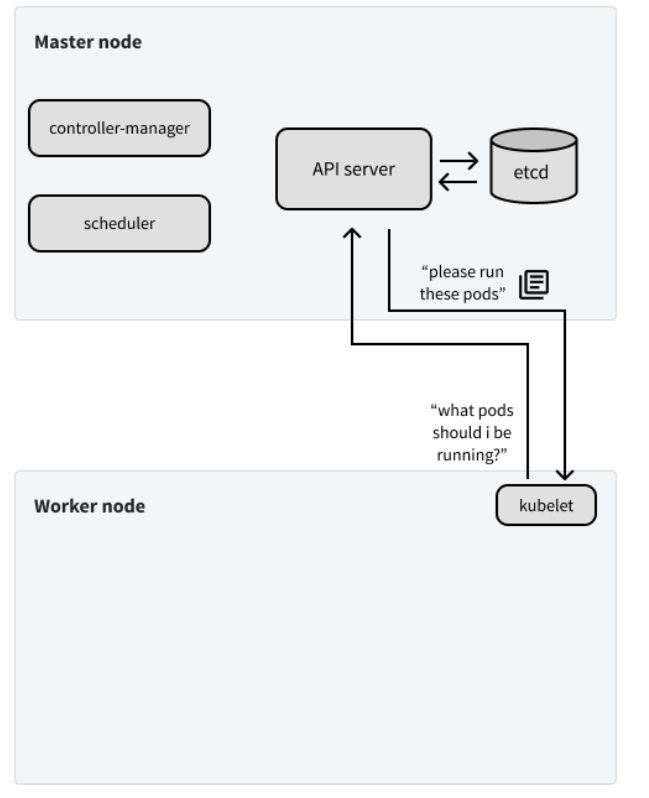
\includegraphics[scale=0.3]{kubelet.png}
	\end{center}
	\item \textbf{kube-proxy}: permette ai container di comunicare tra di loro attraverso i nodi del cluster.
\end{itemize}

\subsection{Conclusione}
Kubernetes non va usato quando:
\begin{itemize}
	\item Il lavoro è leggero e può essere eseguito su una sola macchina
	\item Non è necessario che il servizio sia sempre disponibile
	\item Non sono previste molte modifiche
	\item È progettato in maniera \textit{monolitica}
\end{itemize}
In questi casi è infatti più comodo e veloce usare \textbf{Docker swarm}.
	% !TeX spellcheck = it_IT
\newpage
\section{Datacenter}
Vediamo alcuni esempi di datacenter:
\begin{example}[Google]
	Il datacenter di \hyperref{https://www.youtube.com/watch?v=avP5d16wEp0&list=LLe8YQrC8Io0iIj1IsacdJRA}{}{}{Google} ha impiegati presenti 24h/24h, una sala dedicata al \textit{networking}, un intero piano di server e uno dedicato al \textbf{raffreddamento}.
\end{example}
\begin{example}[UniPi]
	La rete dell'università di Pisa si compone di più di $9000km$ di fibra con una velocità di connessione tra i datacenter (DCI) di $400 Gbit/s$. Inoltre non ha \textbf{Single Point of Failure} ed è ridondante sia a livello fisico che ai livelli L1 e L2.\\
	Il datacenter principale di San Piero a Grado si costituisce di circa 700 nodi e sfrutta un raffreddamento di tipo \textbf{adiabatico}, ovvero sfrutta l'evaporazione dell'acqua per raffreddare l'ambiente nei momenti più caldi. Ha un \textbf{PUE} di 1.2 e una connessione con il \textit{GARR} di $100Gbit/s$.\\
	Utilizza una topologia di tipo \textbf{spine-leaf} per il traffico locale:
	\begin{center}
		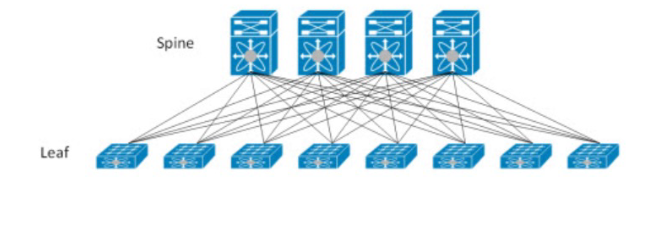
\includegraphics[scale=0.5]{spine_leaf.png}
	\end{center}
\end{example}

\subsection{Energia}
\subsubsection{Consumi}
Nel 2022 i consumi globali dei datacenter sono stati di $460TWh$, circa il $2\%$ del consumo globale, ed è previsto che arrivino a più di $1000TWh$ nel 2026 (il consumo del Giappone).\\
Di tutta questa energia il $40\%$ serve per il \textbf{raffreddamento}.\\
Il posto con la maggiore densità di datacenter è l'Arizona in quanto il costo dell'elettricità è molto basso. Questo perché l'energia usata non è pulita e abbiamo di conseguenza un grosso impatto ambientale.
\subsubsection{PUE}
Il \textbf{Power Usage Effectiveness} misura quanta energia viene usata per componenti non IT all'interno del datacenter (e.g. raffreddamento).
\begin{equation}
	PUE=\frac{P_{IT}+P_{non\_IT}}{P_{IT}} = 1 + \frac{P_{non\_IT}}{P_{IT}}
\end{equation}
\begin{note}
	Il PUE non rappresenta il tasso di energia rinnovabile utilizzata.
\end{note}
\subsection{Management}
La gestione di un datacenter si divide in diversi aspetti:
\begin{itemize}
	\item \textbf{Pianificazione}
	\item \textbf{Installazione} dei rack e delle connessioni
	\item \textbf{Cablaggio}
	\item \textbf{Monitoraggio} dell'infrastruttura
\end{itemize}
\subsubsection{DCIM}
Il \textbf{Data Center Infrastructure Management} si occupa di monitorare in maniera centralizzata l'infrastruttura fisica, in particolare:
\begin{itemize}
	\item Energia
	\item Raffreddamento
	\item Sicurezza
	\item Ambiente
\end{itemize}
Inoltre genera dei \textbf{report} personalizzati e avvisa istantaneamente in caso di \textbf{problemi} all'infrastruttura.
\subsubsection{Sicurezza}
Di seguito alcune cose da \textbf{NON} fare per evitare problemi nel datacenter:
\begin{itemize}
	\item Cavi mal installati
	\item Portare cibi e bevande
	\item Scarsa documentazione
	\item Non tenere traccia di chi ha gli accessi e di quando questi avvengono
	\item Ignorare i rischi di blackout
\end{itemize}
\subsubsection{Outages}
Quando avviene un'interruzione del servizio è importante:
\begin{enumerate}
	\item Essere subito disponibili e concentrati
	\item Gestire bene il panico
	\item Seguire le \textbf{checklist}
\end{enumerate}
Le \textbf{checklist} sono importanti per assicurare \textbf{qualità} nella gestione dell'emergenza e per ridurre la \textbf{responsabilità} dei dipendenti.
\begin{example}[Checklist]
	Un esempio di checklist in caso di incendio:
	\begin{enumerate}
		\item Capire la natura e l'estensione dell'incendio
		\item Usare i sistemi di antincendio a disposizione e se è troppo grosso chiamare subito le autorità ed evacuare
		\item Chiamare le autorità
		\item Evacuare
		\item Se presenti attivare le misure di backup
		\item Appena l'incendio è spento, quantificare i danni
		\item Aggiornare i superiori sulla situazione
	\end{enumerate}
\end{example}

\subsubsection{Continuità e recupero}
Di seguito alcune regole di base per garantire la \textbf{Business Continuity \& Disaster Recovery}:
\begin{itemize}
	\item Mantenere una copia completa dei dati critici almeno a 200km e su una rete elettrica separata
	\item Testare il piano BC/DC
	\item Assicurarsi che eventuali modifiche alla produzione si riflettano sul piano BC/DC
	\item Rendere il piano accessibile e disponibile anche in caso di problemi grossi
	\item Addestrare diverse persone ad eseguire il piano
	\item Ricordare che se qualcosa può andare storto, lo farà
\end{itemize}
\subsection{Iperconvergenza}
Un'infrastruttura può variare in base a quanto vengono virtualizzate le varie parti necessarie (network, server e storage). Ci sono tre casi:
\begin{itemize}
	\item \textbf{Non convergente}: la struttura tradizionale
	\item \textbf{Convergente}: storage e server su macchine separate
	\item \textbf{Iperconvergente}: tutto su un'unica macchina virtualizzata
\end{itemize}
\begin{center}
	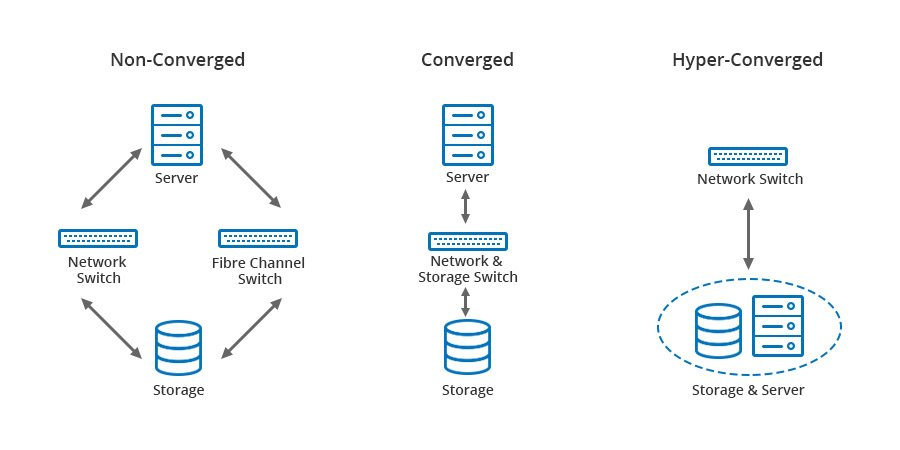
\includegraphics[scale=0.5]{Hyperconvergence.jpg}
\end{center}
	% !TeX spellcheck = it_IT
\newpage
\section{Cloud Edge Continuum}
Con l'aumentare dei dispositivi IoT nella nostra società (e.g. smart cities, power plants, AI), cresce anche la domanda per la potenza di calcolo. \\
Ognuno di questi dispositivi raccoglie dei dati con dei sensori, li processa e poi esegue delle azioni. È proprio la fase di \textbf{lavorazione} dei dati che sta diventando sempre più critica.
\subsection{Implementazioni tradizionali}
\subsubsection{Edge Computing}
I dati vengono processati ai "confini" della rete, garantendo una \textbf{latenza} molto bassa ma limitando di molto la quantità di dati che possono essere processati ed immagazzinati.
\subsubsection{IoT \& Cloud}
I dati vengono inviati e processati nel Cloud, garantendo \textbf{risorse pressoché illimitate} ma aumentando di molto la latenza e causando un overhead in essa. 
\subsection{Cloud Edge Continuum}
Questa implementazione è un ibrido tra le due precedentemente descritte con l'obiettivo di avere il meglio di entrambe: \textbf{latenza bassa}, \textbf{connettività} e \textbf{potenza di calcolo}.\\
Per farlo le applicazioni devono essere: \textbf{containerizzate} e basate su \textbf{microservizi}.
\subsubsection{Posizionamento}
Ogni \textbf{applicazione} ha diverse caratteristiche, tra cui:
\begin{itemize}
	\item Requisiti \textit{hardware}
	\item Requisiti \textit{software}
	\item \textit{QoS}
	\item \textit{Data awareness}
	\item \textit{Sicurezza e affidabilità}
\end{itemize}
mentre l'infrastruttura è \textbf{eterogenea}, \textbf{grande} e \textbf{dinamica}.\\
È necessario capire dove posizionare ogni servizio dell'applicazione, se nell'access point, nel cabinet, nel datacenter o nel cloud. Esistono tre approcci alla soluzione del problema:
\begin{itemize}
	\item \textbf{Machine learning}: prima o poi prenderà una scelta, non per forza corretta. L'infrastruttura è dinamica e difficile da spiegare.
	\item \textbf{Mixed Integer Linear Programming}: trova soluzioni sempre ottimali ma difficile da leggere e da programmare quando sono presenti dati non numerici. Inoltre è lenta da avviare.
	\item \textbf{Ragionamento dichiarativo}: si definiscono i requisiti di un determinato servizio. Il motore di inferenza cerca poi tutte le possibili soluzioni. È facile da leggere e da spiegare.
\end{itemize}

\subsection{Gestione}
Nel mondo di oggi le cose sono in continuo cambiamento. È importante \textbf{monitorare} continuamente le applicazioni e le infrastrutture in modo da avere un ragionamento continuo che permetta di intervenire velocemente.
\end{document}
